% This document is licensed, at your option, under these or any newer versions of these licenses:
% Creative Commons Attribution 3.0 Unported License
% Creative Commons Attribution 4.0 International License
%
% You should have received a copy of the license along with this work. If not, see:
% <http://creativecommons.org/licenses/by/3.0/>
% <http://creativecommons.org/licenses/by/4.0/>

\documentclass{isprs}
\usepackage{subfigure}
\usepackage{setspace}
\usepackage{geometry} % added 27-02-2014 Markus Englich
\usepackage{epstopdf}
\usepackage{url}
\usepackage[dvipsnames]{xcolor}
\usepackage[colorlinks, allcolors=Blue]{hyperref}
%\usepackage[pdfborderstyle={/S/U/W 1}, citebordercolor=purple, urlbordercolor=blue]{hyperref}
%\usepackage{natbib}

\geometry{a4paper, top=25mm, left=20mm, right=20mm, bottom=25mm, headsep=10mm, footskip=12mm} % added 27-02-2014 Markus Englich
%\usepackage{enumitem}

%\usepackage{isprs}
%\usepackage[perpage,para,symbol*]{footmisc}

%\renewcommand*{\thefootnote}{\fnsymbol{footnote}}



\begin{document}

\title{VALIDATION STRATEGY COMPARISON FOR PLS REGRESSIONS}

\author{
 D. Masili\=unas\textsuperscript{a}}

\address
{
	\textsuperscript{a }Wageningen University, Droevendaalsesteeg 3, NL 6708 PB, Wageningen, The Netherlands - dainius.masiliunas@wur.nl
}

\icwg{}   %This field is NOT optional after all.

\abstract
{
To be added.
}

\keywords{To, Be, Determined}

\maketitle

\section{INTRODUCTION}\label{INTRODUCTION}

Validation is an important step in the model creation process, as it determines how well the model performs in practice and whether it is reliable enough for the required use-case. Validation also gives insight into how many samples of the population need to be taken to achieve a certain model accuracy level.

There are two types of model validation: holdout (true, conventional) validation and cross-validation. In holdout validation, the total sample set is divided into two subsets: a training (model building) and validation (test) sets. Only the training set is used for creating the model. The validation set is put aside, in order to more realistically assess the model performance after it is created. The drawback to holdout validation is that by holding back some of the samples, the sample size from which a model is derived becomes smaller, and thus the model accuracy suffers. In order to achieve the same level of accuracy as when not doing holdout validation, extra samples equal to the validation set size need to be collected, which can be a costly and time-consuming task.

In contrast, in cross-validation, all available samples in the model are used. The validation step is made possible by temporarily splitting the full sample set into training and validation sets, as in holdout validation, but it is repeated a number of times with different ways of splitting, so that every sample goes in both the training and validation set at least once. Then a summary statistic is calculated and used to determine the model accuracy. The drawback to cross-validation is that since all samples are used in the model, it cannot be utilised as a way to optimise the model for better external validity by dropping samples without worthwhile information from the training set. In addition, cross-validation tends to produce overly optimistic results, since the model takes the samples used for validation into account.

There are numerous strategies for splitting the samples into training and validation sets for each of the validation types. There have been studies comparing them \cite{clark2003boosted}, but to date there has not been a comprehensive study comparing validation methods when applied specifically to the hyperspectral models used in earth observation. In this paper, the effectiveness of a number of different cross-validation and holdout validation strategies on Partial Least Squares Regression (PLSR) models have been assessed. In particular, we take a look at how cross-validation techniques influence the selection of the number of components to use when building the model, and how model accuracy scales with sample size when different holdout validation techniques are applied.

\section{METHODS}\label{sec:METHODS}

\subsection{Cross-validation strategies}\label{sec:Cross-validation strategies}

In order to assess how cross-validation techniques influence the selection of the number of components, the R package \textit{plsr} was used, specifically the function \textit{validationplot()} with different cross-validation parameters available in the package. The validation plots show how the root mean square error of prediction (RMSEP) changes with an increasing number of latent vectors used in the regression.

Tested cross-validation sampling stategies were: Leave-one-out (LOO), random, interleaved and consecutive sampling, as well as the mean of 100 Monte Carlo runs of random sampling. For sampling strategies other than LOO, the full data set was divided into two subsets validated against each other (2-fold cross-validation). If the number of subsets \textit{k} is increased, the result gets closer and closer to LOO cross-validation result (see figure \ref{fig:interleaved-group-sizes}), and at 16 groups is already very close to LOO.

\begin{figure}[ht!]
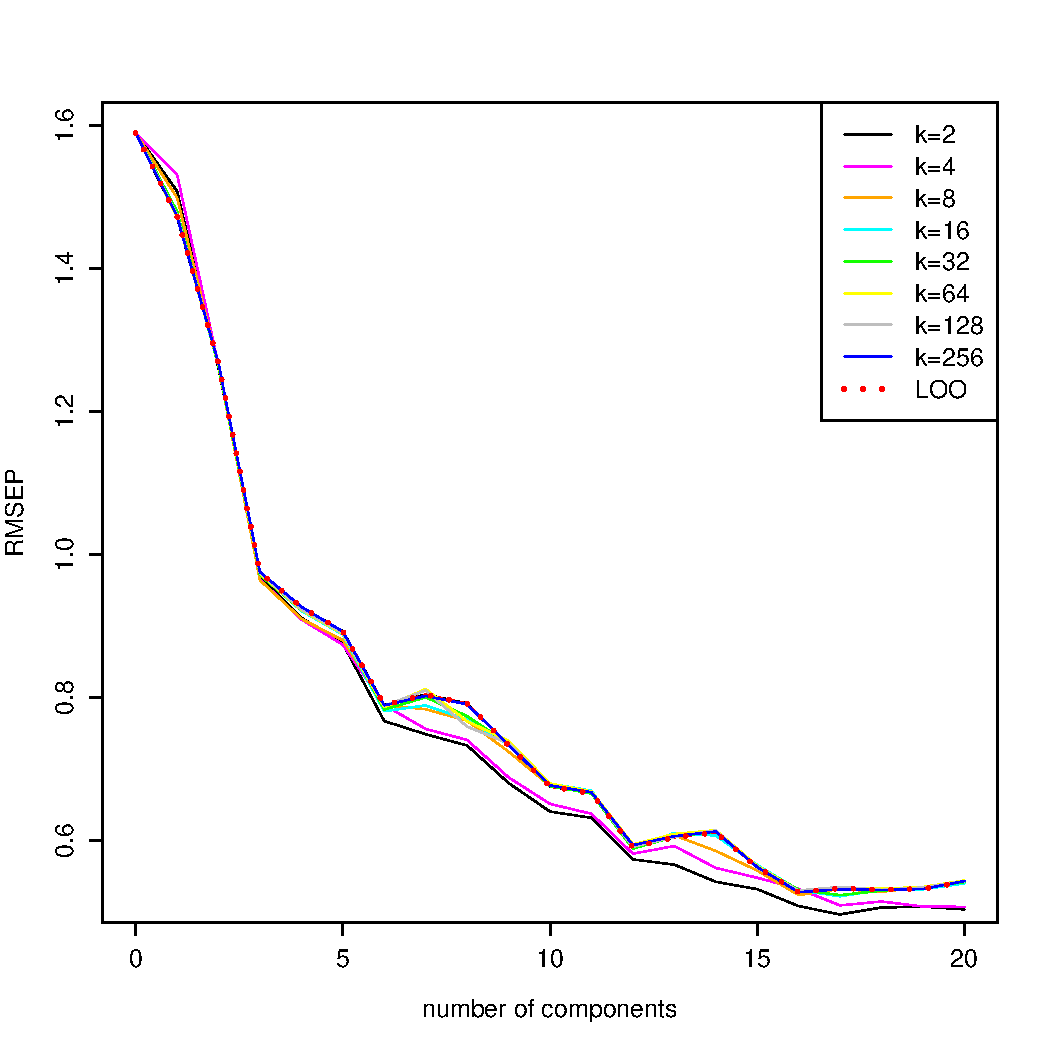
\includegraphics[width=1.0\columnwidth]{../script/output/interleaved-group-sizes.pdf}
\begin{center}
    \caption{Interleaved sampling cross-validation result with an increasing number of cross-validation subsets \textit{k}, compared to Leave-one-out validation.}
    \label{fig:interleaved-group-sizes}
\end{center}
\end{figure}

\subsection{Holdout validation strategies}\label{sec:Holdout validation strategies}

For assessing holdout validation techniques, samples were split into training and validation sets manually for random without replacement, random with replacement (bootstrapping) and stratified random sampling. For the respective Monte Carlo simulations, the splitting into different sets was repeated 100 times, and the result was averaged over all runs. For Kennard-Stone sampling, the R package \textit{inspectr} was used to generate the validation sample set, based on the Kennard-Stone algorithm \cite{kennard1969computer}. For OptiSim sampling \cite{clark1997optisim}, the latest in-development code from the \textit{inspectr} package was used. OptiSim sampling was run using clusters of 4 samples (k = 4), since studies have shown that this setting generally performs the best on hyperspectral datasets \cite{clark2003boosted}.

Two strata were used for stratified random sampling: one stratum included samples with pH below the median pH for all samples (6.11), and the other included all samples equal or above the median. The strata were chosen as such because pH distribution among samples is bimodal, with fewer values around the median value (which is also close to the neutral pH value of 7). Splitting the strata at the median allows for balanced strata, without the need to use bootstrapping or drop samples.

The validation was repeated twice: the first time the validation set used all unused samples from the same Netherlands soil dataset as the training set, whereas the second time the external Australian soil dataset was used for validation.

In addition, the above was repeated twice, using different number of latent vectors for the PLS regression, in order to see how the choice of the number of latent vectors from cross-validation impacts the PLS regression and its holdout validation.

\subsection{Data}\label{sec:Data}

The model used for this paper was created by using the Netherlands soil spectra dataset, using the \textit{plsr} package. For assessing the external performance of the resulting models, the Australian soil spectra dataset \cite{rossel2010using}, provided in the \textit{inspectr} package, was used as a validation set.

\section{RESULTS}\label{sec:RESULTS}

\subsection{Cross-validation strategies}\label{sec:Cross-validation strategies 2}

The cross-validation sampling strategies for the Netherlands soil dataset used produced similar results to one another, with the overall shape of the curve when an increasing number of latent vectors is used for the regression being the same across all the tested strategies except for consecutive sampling (see figure \ref{fig:cv}). Consecutive sampling resulted in higher RMSE values than other strategies, although the minimum RMSE value of 0.70 was still for 16 latent vectors, just like with LOO cross-validation (in which case the RMSE was 0.53).

The random sampling strategy results in an unstable minimum RMSE value, since the full data set is split into two subsets randomly. Running Monte Carlo simulation for it results in more stable results (depending on the number of runs) which are also closer to those obtained by LOO cross-validation. The standard deviation of the Monte Carlo simulation was 0.02 RMSE.

Of all the cross-validation strategies tested, the lowest RMSE values were obtained using interleaved cross-validation, however, whether interleaved cross-validation is suitable for use depends on the way the dataset is laid out. Monte Carlo simulation of random sampling resulted in the second lowest RMSE values, and LOO cross-validation had third lowest RMSE values.

Given the cross-validation results, holdout validation analysis was first done using 16 latent vectors, and then repeated using 6 latent vectors, since it is the first local RMSE minimum for both LOO and consecutive cross-validation results.

\begin{figure}[ht!]
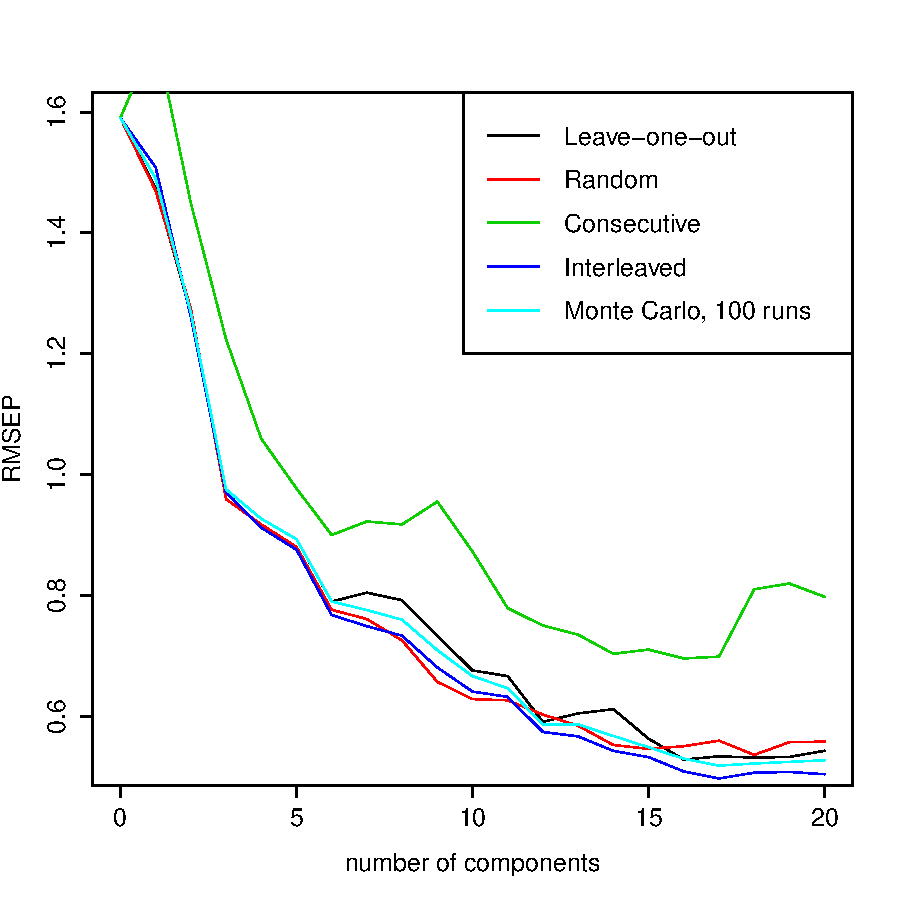
\includegraphics[width=1.0\columnwidth]{../script/output/cv.pdf}
\begin{center}
    \caption{PLSR validation plot when using different sampling strategies.}
    \label{fig:cv}
\end{center}
\end{figure}

\subsection{Holdout validation strategies}\label{sec:Holdout validation strategies 2}

\subsubsection{16 latent vectors, Netherlands soil validation:}\label{sec:NL16}

When comparing how RMSE values change as the number of samples used in the PLS regression increases using various holdout validation strategies, with validation samples from the same dataset, we can see a typical pattern of RMSE gradually going down until it becomes stable at around 150 samples for most sampling strategies (see figure \ref{fig:rmse-nl-16}).

Just like with cross-validation, sampling methods that have a random component to them (simple and stratified random sampling as well as bootstrapping) are not consistent when performed only once and require Monte Carlo simulations to become stable. The standard deviation of these methods is generally higher towards the edges, that is, when either the training or the validation set sizes become low.

Stratified and simple random sampling after 100 Monte Carlo runs result in very similar RMSE values, whereas bootstrapping gives slightly higher RMSE values.

Kennard-Stone sampling results in the lowest RMSE values, no matter the sample size. Optisim sampling performs very poorly when the training set size is very low, but quickly gets better as more samples are added to the training set, even overtaking Kennard-Stone sampling at 56 samples in the training set. However, the decrease in RMSE when adding more samples to the model beyond that is no longer any better than when using simple or stratified Monte Carlo methods.

The RPD values exceeded 3 for Kennard-Stone sampling starting from 132 samples in the training set (with a maximum of 3.58 RPD at 240 samples), and never for the other sampling methods (not counting random-based sampling without Monte Carlo), although at the maximum of 256 samples, Monte Carlo simple random sampling achieved 2.98 RPD.

\begin{figure}[ht!]
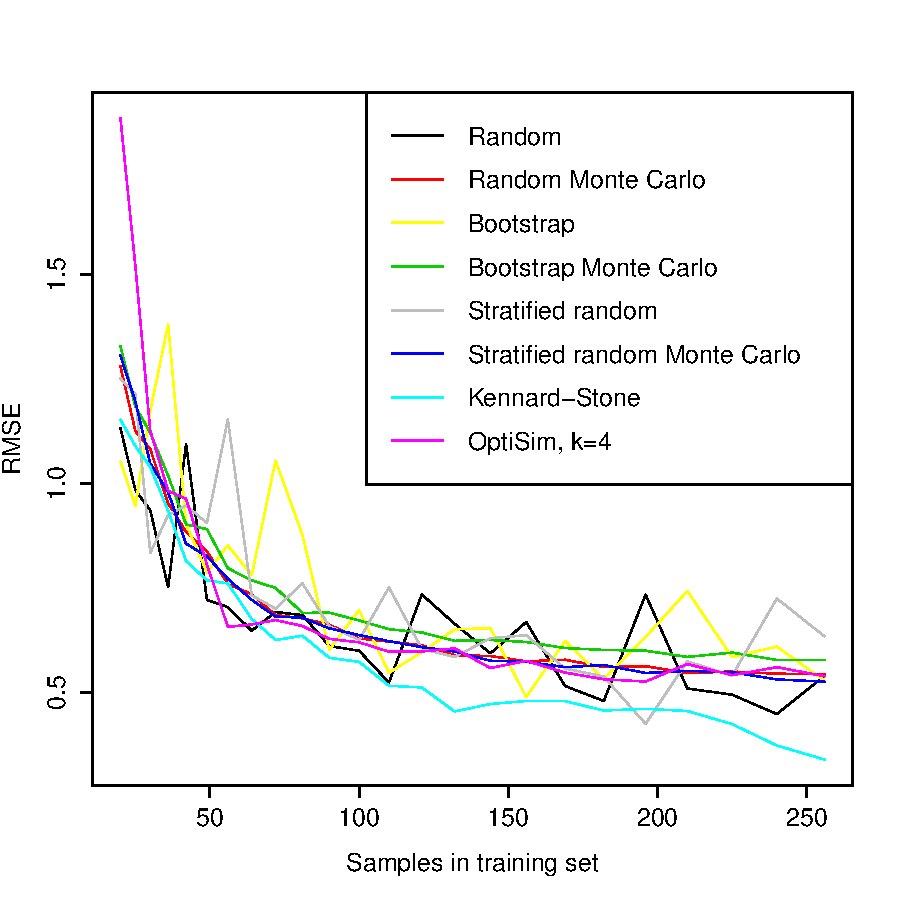
\includegraphics[width=1.0\columnwidth]{../script/output/rmse-nl-16.pdf}
\begin{center}
    \caption{Performance of various holdout validation strategies as the training set size increases. The validation set consists of all samples from the same dataset not used in the training set, number of latent vectors used is 16.}
    \label{fig:rmse-nl-16}
\end{center}
\end{figure}

\subsubsection{16 latent vectors, Australian soil validation:}\label{sec:AU16}

The results when using an independent validation set are completely different (see figure \ref{fig:rmse-au-16}). Most sampling strategies produce a flat line for RMSE, meaning that adding more samples into the model has no effect at all on the pH prediction accuracy in Australian soils.

Kennard-Stone sampling, when the training set is small (less than 100 samples), consistently performs better than random sampling methods, but as the training set increases, it is no longer distinguishable from the random sampling methods.

RPD values never exceeded 0.4 even when the single runs of random sampling methods are taken into account. Thus while the internal prediction of the model when using random Monte Carlo and Kennard-Stone sampling is good enough for screening, the external predictive power of the same model is extremely poor.

\begin{figure}[ht!]
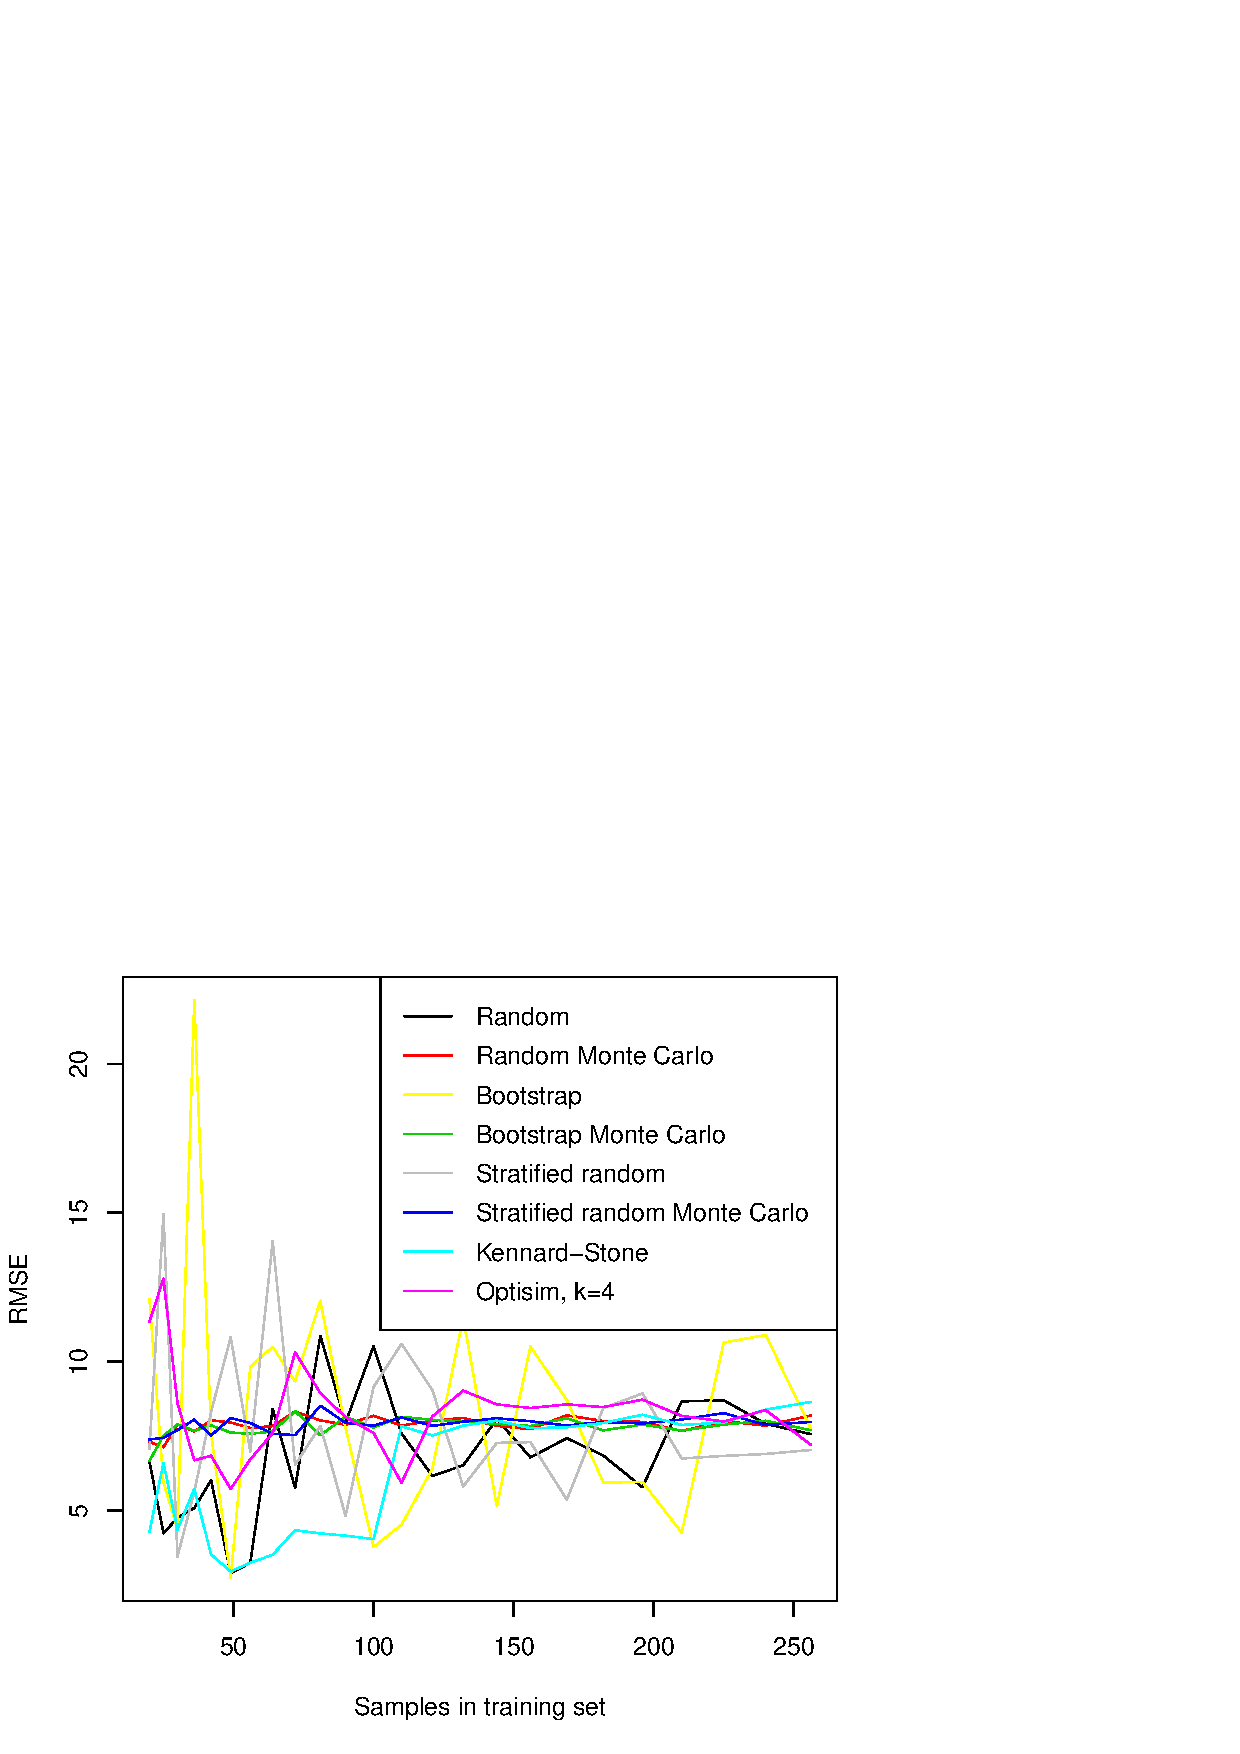
\includegraphics[width=1.0\columnwidth]{../script/output/rmse-au-16.pdf}
\begin{center}
    \caption{Performance of various holdout validation strategies as the training set size increases. The validation set consists of all samples in the Australian soil dataset, number of latent vectors used is 16.}
    \label{fig:rmse-au-16}
\end{center}
\end{figure}

\subsubsection{6 latent vectors, Netherlands soil validation:}\label{sec:NL6}

When the analysis is repeated for a model using 6 latent vectors, using the Netherlands data for validation, the general pattern stays the same as for 16 latent vectors (see figure \ref{fig:rmse-nl-6}). The main differences are the RMSE values, which are higher as shown in the cross-validation phase, and the patterns for Kennard-Stone sampling as well as Optisim.

At a low number of samples in the training set, Kennard-Stone sampling performs worse than any other sampling method (not counting single random realisations), but evens out at 125 training set samples and has lower RMSE values than other sampling methods as the number of training samples increases past 150. The pattern for Optisim sampling is contrary to that of Kennard-Stone, with Optisim performing the best when the training set is small and worse than the random methods when the training set is larger than 150 samples.

As expected, none of the sampling methods ever achieve an RPD close to 3 when using only 6 latent vectors, with the maximum achieved by Kennard-Stone sampling at 2.12.

\begin{figure}[ht!]
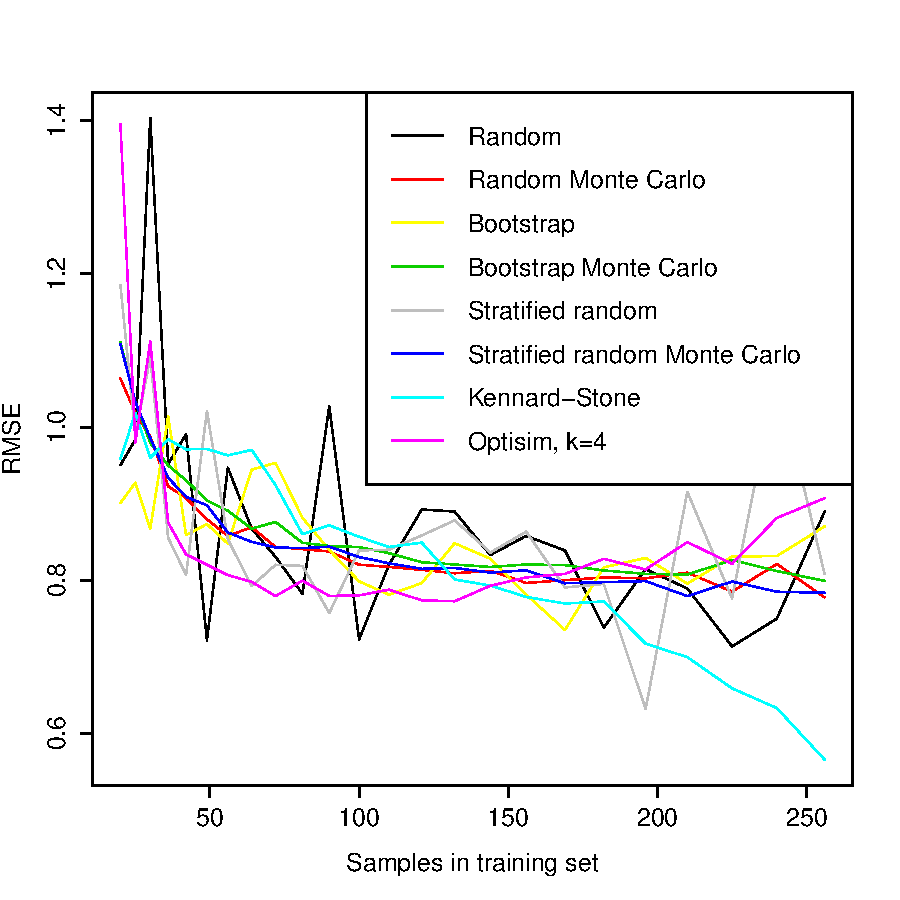
\includegraphics[width=1.0\columnwidth]{../script/output/rmse-nl-6.pdf}
\begin{center}
    \caption{Performance of various holdout validation strategies as the training set size increases. The validation set consists of all samples from the same dataset not used in the training set, number of latent vectors used is 6.}
    \label{fig:rmse-nl-6}
\end{center}
\end{figure}

\subsubsection{6 latent vectors, Australian soil validation:}\label{sec:AU6}

When the Australian dataset is used for validation at 6 latent vectors, there are notable changes from when 16 components were used (see figure \ref{fig:rmse-au-6}). The RMSE values are overall lower. The random sampling methods in this case show a small decrease in RMSE when the training set size is increased up to 50, but flattens out after that.

Kennard-Stone sampling shows an even more pronounced inverse curve than in the 16 latent vector case, with the RMSE increasing as more samples are added into the training set, with lower RMSE values than other sampling methods. On the other hand, Optisim starts out performing worse than the other sampling methods, but the RMSE value gets progressively closer to that of the random methods. The highest RPD value achieved by Kennard-Stone sampling is 0.89 at only 20 samples in the training set.

\begin{figure}[ht!]
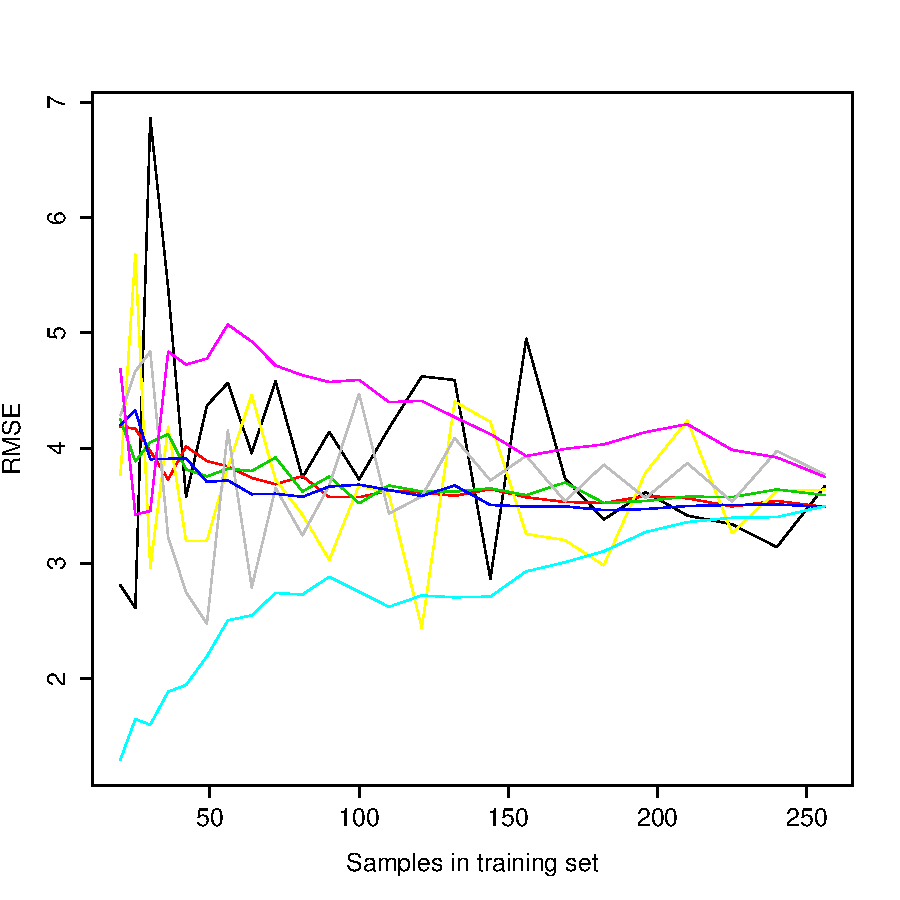
\includegraphics[width=1.0\columnwidth]{../script/output/rmse-au-6.pdf}
\begin{center}
    \caption{Performance of various holdout validation strategies as the training set size increases. The validation set consists of all samples in the Australian soil dataset, number of latent vectors used is 6. The colours represent the same methods as in previous graphs.}
    \label{fig:rmse-au-6}
\end{center}
\end{figure}

\section{DISCUSSION}\label{sec:DISCUSSION}

\subsection{Cross-validation strategies}\label{sec:Cross-validation strategies 3}

From the cross-validation strategies tested, each has its own peculiarities. Random sampling gives results that are not stable, therefore at low \textit{k} it is not suitable for determining the optimal number of latent vectors to use in the regression by itself. However, since for the dataset used the standard deviation of random sampling was low, using Monte Carlo random sampling, even with relatively low number of runs, is an option. Generally it gives results very similar to that of Leave-one-out cross-validation.

Leave-one-out cross-validation result itself is deterministic, however, it requires recalculating the PLS regression for every sample included in the model, thus it takes more time than all other cross-validation strategies tested (aside from Monte Carlo, which can have an arbitrarily high number of runs).

Interleaved sampling in this case gave good results, was fast and deterministic, however, it depends on the way the dataset is organised. Often times datasets are ordered by how the samples were taken, for instance, by starting collecting samples at one end of an area and finishing at the other. However, if every or nearly every other sample was taken from an area with different properties, then the subsets of interleaved samples will no longer be representative of one another and result in unusually high RMSE values. Therefore choosing interleaved sampling with no \textit{a priori} knowledge of how the dataset was made is risky and may lead to an incorrect choice of latent vectors to use.

That is what happened in this case with consecutive sampling. If there is a gradient or a jump in values in the dataset due to physical properties at one end of an area being different from the other end of it, consecutive sampling will produce subsets that are not representative of one another.

\subsection{Holdout validation strategies}\label{sec:Holdout validation strategies 3}

From the holdout validation strategies tested, Kennard-Stone sampling performed the best in all cases. This is due to the Kennard-Stone algorithm selecting samples of highest difference from the dataset first. Since those samples have the largest variation, they also hold most of the information about the data collected, and the rest of the samples (which are less extreme) are used for validation, thus resulting in a consistently lower RMSE. However, calculating the differences between each of the samples takes a lot of time and computing power.

Stratified random sampling generally performed the same as simple random sampling. This is likely to be due to the rather simplistic method of stratifying chosen. If there was data about the soil type that each spectrum represented, and it was used to divide the dataset into strata, then the performance between simple and stratified sampling might have been different.

Bootstrap sampling performed worse than random sampling without replacement, since samples were duplicated. This acts opposite of the Kennard-Stone method, with more redundant data going into the training set, and the model overfitting those samples, compared to the remaining ones (that were used for validation).

When the Australian soil dataset was used for validation, the model fit was poor for all sampling methods when using 16 latent vectors in the model, in stark contrast with the model fit when the same dataset was used for validation. This indicates that the model is overfitting for the samples in the training dataset, resulting in little to no predictive power outside the training dataset. This is expected, since 16 latent vectors is a very high number for typical applications, and the last latent vectors are likely to not contain any information useful for external prediction at all.

Unfortunately, none of the cross-validation strategies indicated such a problem, with most of them agreeing that 16 latent vectors is the optimal choice. This confirms that cross-validation tends to be overoptimistic. Therefore choosing a lower number of latent vectors than it might appear optimal from cross-validation graphs is important, if external prediction is the goal of the PLSR model. In this case, some of the cross-validation graphs indicated a small local minimum at 6 latent vectors, thus the analysis was repeated for that number of latent vectors.



{%\footnotesize
	\begin{spacing}{0.9}% tune the size by altering the parameter
		\bibliography{AEO-paper}
	\end{spacing}
}

\section*{APPENDIX}\label{APPENDIX}

The R code used to carry out the analysis for this paper is available online, at:

\url{https://github.com/GreatEmerald/AEO-validation-paper}

\end{document}
